%*************************************************************************
\section{Voraussetzung und Installation}
%*************************************************************************

SiLift ist als \textit{Eclipse-Feature} unter folgender \textit{Update-Site} erhältlich:\\ \url{http://pi.informatik.uni-siegen.de/Projekte/SiLift/updatesite}.\\

\textbf{Hinweis:} Vergewissern Sie sich, ob ihr Eclipse die notwendigen Voraussetzungen erfüllt. 
Eine Liste der benötigten Plugins ist unter \url{http://pi.informatik.uni-siegen.de/Projekte/SiLift/download.php} zu finden.
Bitte beachten Sie dabei die entsprechenden Hinweise zu den jeweiligen Versionen.\\

Sofern alle Voraussetzungen erfüllt sind, kann SiLift wie gewohnt über den Menüpunkt \texttt{Help} $\triangleright$ \texttt{Install New Software...} installiert werden (Abb. \ref{eclipse-install_new_software}).
\begin{figure}[H]
\centering
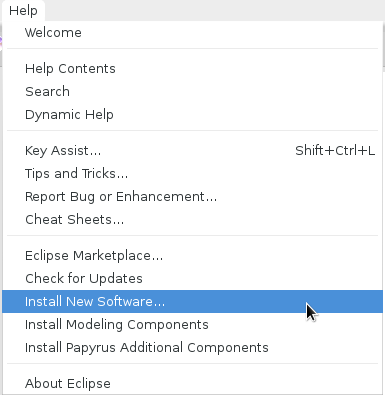
\includegraphics[width=0.25\textwidth]{requirements/graphics/eclipse-install_new_software.png}
\caption{Eclipse: Install New Software...}
\label{eclipse-install_new_software}
\end{figure}

Es sollten Ihnen vier Kategorien angezeigt werden (vgl. Abb. \ref{eclipse-install_silift}). 

\begin{figure}[H]
\centering
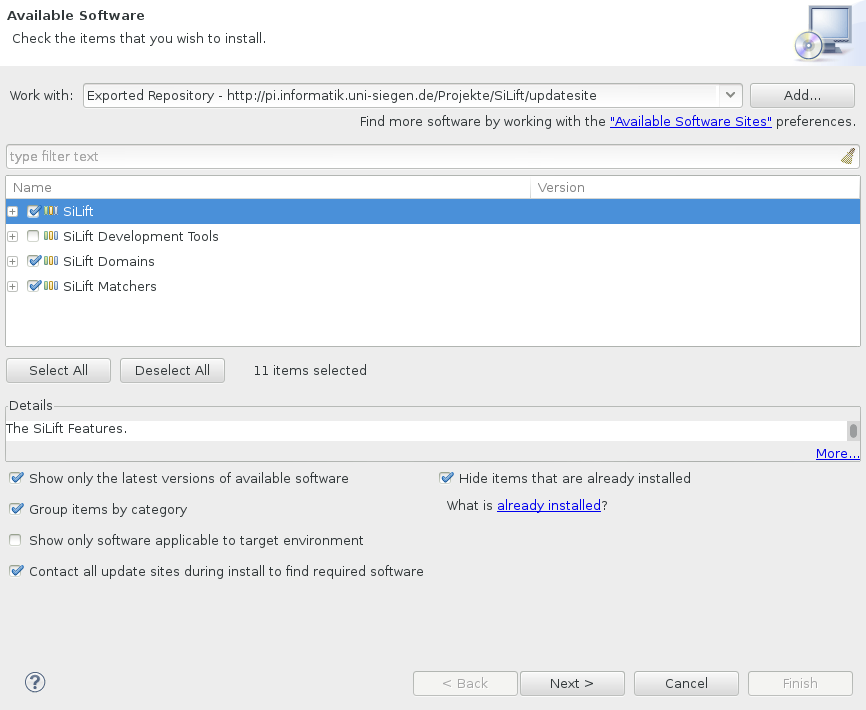
\includegraphics[width=0.5\textwidth]{requirements/graphics/eclipse-install_silift.png}
\caption{SiLift Update Site}
\label{eclipse-install_silift}
\end{figure}

Für die folgenden Tutorials benötigen wir alle Features aus der Kategorie \texttt{SiLift},  das Feature \texttt{SiLift Ecore Domain} aus der Kategorie \texttt{SiLift Domains}, sowie den \texttt{SiLift Named Element} und \texttt{SiLift UUID Matcher} aus \texttt{SiLift Matchers}. Sie könnenn aber auch wie in Abbildung \ref{eclipse-install_silift} die kompletten Kategorien auswählen. Danach klicken Sie auf \texttt{Next} und folgen dem Installationsassistenten.\\

\textbf{Hinweis}: Generell unterstützt SiLift alle \textit{EMF-basierten} Modellierungsprachen, sofern die ent\-sprech\-enden \textit{Editieroperationen} implementiert wurden.
In der aktuellen Version stehen diese bereits für \textit{Ecore-} und \textit{Feature-Modelle} zur Verfügung.\footnote{Informationen zur Integration weiterer Modelltypen finden Sie im \textbf{SiLift - Benutzerhandbuch für Entwickler}.}
